\section{Durchführung}
\FloatBarrier
\label{sec:Durchführung}
\subsection{Messung der Geschwindigkeit des Wagens}
\label{sec:speedygonzales}
\begin{figure}
	\centering
	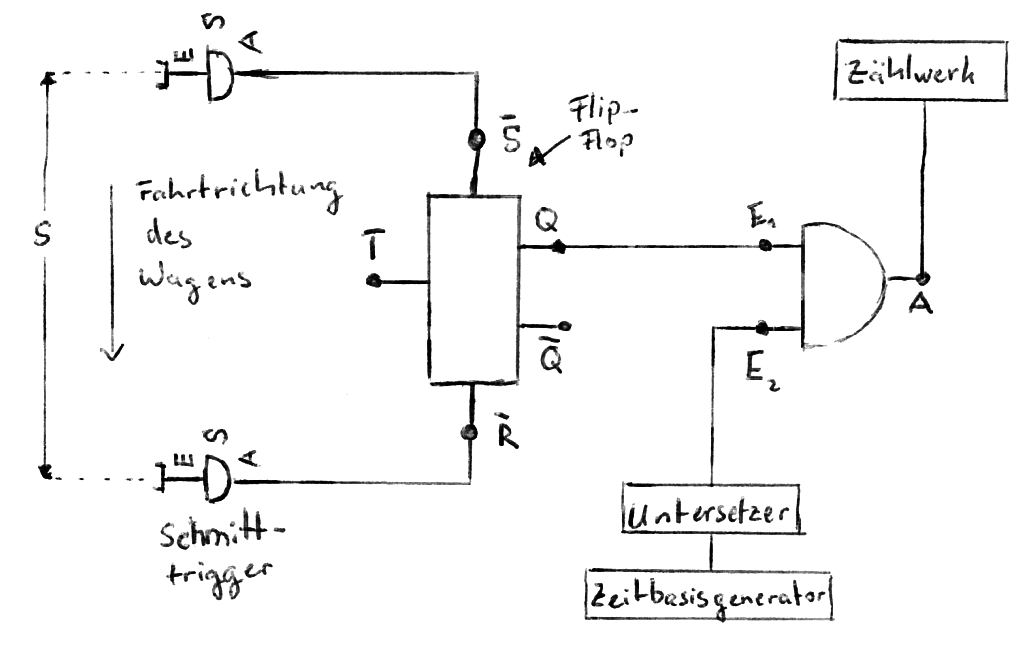
\includegraphics[width=0.75\textwidth]{Bilder/geschwindigkeit_schaltung.png}
	\caption{Prinzipieller Aufbau zur Untersuchung der Wagengeschwindigkeit.}
	\label{fig:wagen} %eventuell ersetzen mit den eigenen Schaltplänen, kann ich am we mal machen
\end{figure}
Zur Messung der Geschwindigkeit des Wagens wird die Schaltung wie in Abbildung \ref{fig:wagen} aufgebaut.\\
Zur Bestimmung der Geschwindigkeit ist eine präzise Messung der Fahrzeit des Wagens zwischen den beiden Lichtschranken auf der Strecke $s$ nötig.\\
Daher wird beim Durchfahren der ersten Lichtschranke die Zeitmessung gestartet und beim Durchfahren der zweiten Lichtschranke die Zeitmessung gestoppt.
Beim Durchfahren der ersten Lichtschranke sendet diese über einen Schmitt-Trigger einen kurzen \textbf{LOW}-Impuls. Dieser schaltet über den $\bar{S}$-Eingang einer bistabilen Kippstufe den $Q$-Ausgang auf \textbf{HIGH}-Potential.
Vom $Q$-Ausgang wird das Signal an ein AND-Gatter geleitet,
an dessem zweiten Eingang der Untersetzer mit dem Zeitbasisgenerator angeschlossen ist. \\
Solange am $Q$-Ausgang des Flip-Flops ein \textbf{HIGH}-Potential anliegt, gelangen die durch den Zeitgeber erzeugten Schwingungen in das Zählwerk.
Die Zeitmessung wird gestoppt, indem das \textbf{LOW}-Signal an der zweiten Lichtschranke  bei der Durchfahrt des Wagens auf den $\bar{R}$-Eingang der bistabilen Kippstufe gegeben wird,
sodass am Ausgang $Q$ das Potential auf \textbf{LOW} geändert wird. Die Torstufe (realisiert als AND-Gatter) wird geschlossen und die Schwingungen erreichen nicht mehr das Zählwerk.\\
Am Zählwerk kann die benötigte Fahrzeit nun direkt abgelesen werden.\\
Es werden für jeden Gang des Antriebsmotor des Wagens jeweils 5 Messungen für den Hin- und Rückweg durchgeführt. \\
Die Distanz $s$ wird mit einem Maßband ausgemessen.

\FloatBarrier
\subsection{Messung der Frequenz der Schallwelle bei ruhendem Lautsprecher}
\label{sec:schall} %zu faul zum ändern
Die Messung der Frequenz der Schallwelle bei ruhendem Lautsprecher wird mittels der in Abschnitt \ref{sec:frequenz} erklärten Schaltung ermittelt.
Diese wird hier manuell ausgelöst und dient lediglich dazu, dass die Schwingungen des Zeitbasisgenerators nur für eine fest definierte Zeit gezählt werden.\\
Die Messzeit wird am Untersetzer zu $\SI{1}{\second}$ eingestellt. Am Zählwerk kann somit direkt die Frequenz $\nu_{\mathrm{0}}$ in $\si{\per\second}=\si{\Hz}$ abgelesen werden.\\
Die Messung wird zehnmal wiederholt.
\subsection{Messung der Schallgeschwindigkeit über die Wellenlänge}
Die Schallgeschwindigkeit bei Zimmertemperatur lässt sich bestimmen über die Kenntnis der Frequenz $\nu_{\mathrm{0}}$ des ruhenden Lautsprechers und der Wellenlänge $\lambda$ der Schallwelle.\\
Die Wellenlänge wird über \textbf{LISSAJOUS-Figuren} bestimmt.
Diese entstehen, wenn auf beide Achsen eines Oszilloskops Schwingungen gegeben werden. Dazu wird auf die X-Achse des Oszilloskops das verstärkte Ausgangssignal des Mikrophons und auf die Y-Achse das Signal des Sinusgenerators gegeben.\\
Jede Entartung der \textbf{LISSAJOUS-Figuren} zu einer Geraden stellt eine Phasenverschiebung von $\pi$ zwischen den beiden auf den Achsen gegebenen Schwingungen dar.\\
Mittels der Mikrometerschraube lässt sich, wie ersichtlich in Abbildung \ref{fig:lisa}, der Abstand zwischen Mikrophon und Lautsprecher variieren.
Für jede Entartung des Oszilloskopbildes zu einer Geraden wird anhand
der Maßskala an der Mikrometerschraube die Differenz zwischen zwei Entartungen bestimmt. Diese entspricht der halben Wellenlänge $\frac{\lambda}{2}$.\\
Mittels der bereits in Abschnitt \ref{sec:schall} bestimmten Frequenz der Schallwelle kann jetzt die Schallgeschwindigkeit bestimmt werden.

\begin{figure}
	\centering
	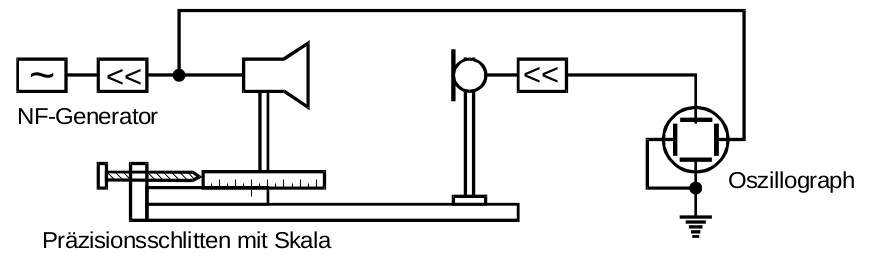
\includegraphics[width=0.9\textwidth]{Bilder/lissajou.png}
	\caption{Aufbau zur Messung der Schallgeschwindigkeit bei Raumtemperatur. \cite{Anleitung}}
	\label{fig:lisa}
\end{figure}

\FloatBarrier
\subsection{Messung der Frequenz der Schallwelle bei bewegter Quelle}
\label{sec:frequenz}
In Abbildung \ref{fig:delphin} ist der prinzipielle Aufbau zur Bestimmung der Frequenz $\nu_{\mathrm{Q}}$ bei bewegter Quelle dargestellt.\\
Der Wagen mit dem Lautsprecher bewegt sich relativ zum Empfänger mit den in Abschnitt \ref{sec:speedygonzales} bestimmten Geschwindigkeiten.\\
Jede Messung wird erneut für jeden Gang des Antriebmotors jeweils fünfmal für den Hin- als auch den Rückweg durchgeführt.
Das Zählwerk zählt genau eine Sekunde lang die Schwingungen der Schallquelle, welche am Empfänger eintreffen. Es wird die Frequenz der Schallwelle, welche am Empfänger eintrifft, auf dem Zählwerk ausgegeben.
zur Steuerung der Schaltung wird das \textbf{LOW}-Signal, welches beim Durchfahren des Wagens durch die Lichtschranke erzeugt wird, auf den $\bar{S}$-Eingang einer bistabilen Kippstufe gegeben, sodass deren $Q$-Ausgang auf \textbf{HIGH}-Potential gestellt wird.
Dieses \textbf{HIGH}-Signal wird genutzt, um zwei Torstufen zu öffnen.
Eine der beiden Torstufen verbindet hierbei den Empfänger mit dem Zählwerk.
Die am Mikrophon registrierte Sinusschwingung wird zunächst allerdings noch über einen Signalwandler in eine $TTL$-Rechteckschwingung umgewandelt, bevor das Signal über die Torstufe auf das Zählwerk gegeben wird.
Die zweite Torstufe dient in der vorliegenden Schaltung der Steuerung der Zeitmessung.
Auf dem zweiten Eingang der zweiten Torstufe wird das Signal des Zeitbasisgenerators aufgegeben.
Da der Ausgang der zweiten Torstufe (auch hier erneut realisiert über ein AND-Gatter) an den Untersetzer angeschlossen ist, muss dieser nur noch so eingestellt werden, dass genau nach einer Sekunde ein Signal
zur weiteren Steuerung der Schaltung weitergegeben wird.\\
Da der Zeitbasisgenerator jede Mikrosekunde einen Schwingungsimpuls sendet, also $10^6$ Impulse pro Sekunde, muss der Untersetzer auf $10^6$ gestellt werden (Der Untersetzer zählt die Anzahl der eintreffenden Impulse, sobald der zuvor festgelegte Wert erreicht ist, sendet der Untersetzer einen \textbf{HIGH}-Impuls).\\
Der durch den Untersetzer gesendete \textbf{HIGH}-Impuls wird auf den $T$-Eingang der bistabilen Kippstufe gegeben. Da die bistabile Kippstufe bei fallender Flanke (von \textbf{HIGH} nach \textbf{LOW}) am \textbf{T}-Eingang den Status am \textbf{Q}-Ausgang ändert, wird dieser auf \textbf{LOW} gesetzt und beide Torstufen der Schaltung deaktiviert.
Am Zählwerk kann die Frequenz $\nu_{\mathrm{Q}}$ jetzt direkt abgelesen werden.

\begin{figure}
	\centering
	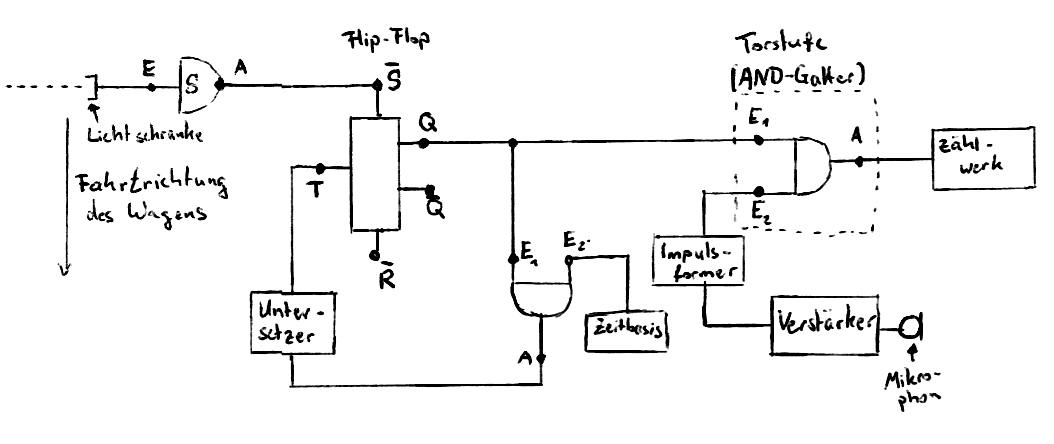
\includegraphics[width=0.9\textwidth]{Bilder/frequenzmessung_schaltung.png}
	\caption{Aufbau zur Messung der Frequenz bei bewegter Quelle.}
	\label{fig:delphin}
\end{figure}

\FloatBarrier
\subsection{Messung der Frequenz über die Schwebungsmethode}
Die Messung der Frequenz über die Schwebungsmethode erfolgt mit nahezu dem gleichen Aufbau wie im vorherigen Abschnitt.\\
Allerdings wird nun der Lautsprecher direkt neben dem Empfänger montiert.
Auf dem Wagen wird stattdessen ein Reflektor montiert. Dieser bewegt sich bezüglich des ruhenden Empfängers mit der Geschwindigkeit $2v$.
Der Empfänger nimmt jetzt sowohl die direkte Schallwelle des Lautsprechers, als auch die reflektierte Schallwelle auf.
Somit entsteht aus der Überlagerung der direkt erzeugten und der reflektierten Schallwelle eine Schwebung.\\
Damit nur die Schwebung gemessen wird, muss vor den Signaleingang des Mikrophons im Aufbau \ref{fig:delphin} ein Tiefpass geschaltet werden.\\
Erneut werden für jeden Gang für Hin-und Rückweg jeweils fünf Werte aufgenommen.
